\chapter{Análise e discussão dos resultados}

\section{Bomba de infusão}
\label{sec:secao_analise_bomba}
O desenvolvimento desse sistema foi dividido em algumas partes: cálculo do intervalo de tempo entre infusões basais e cálculo dos passos necessários. O cálculo do intervalo de tempo entre as infusões basais é executado após a inicialização da bomba, desde que já exista um prévia configuração da quantidade de insulina para a hora em questão. Essa funcionalidade tem a responsabilidade de injetar a quantidade de insulina de forma continua, ou seja, caso a bomba seja desligada não haverá alteração na taxa de injeção para compensar o tempo parado. Testes foram realizados, sem interrupções, levando em conta que a quantidade de infusão mínima é de 0,1 unidades de insulina. A Figura \ref{fig:testeinsulina} representa o resultados dos cálculos e quantidade de insulina injetada.

O objetivo desse teste é verificar o número de infusões de quantidade mínima de insulina que a bomba deveria executar e número de infusões que a bomba efetivamente executou. De acordo com a quantidade de insulina requerida para cada hora. Os testes realizados tiveram duas situações distintas, quando feita a divisão da quantidade de tempo (em segundos) da hora corrente pela quantidade de infusões basais necessárias:

\begin{itemize}
\item Divisão resulta em um intervalo entre infusões com valor inteiro;
\item Divisão resulta em um intervalo entre infusões com valor decimal.
\end{itemize}

\begin{figure}[htp]
	\centering
	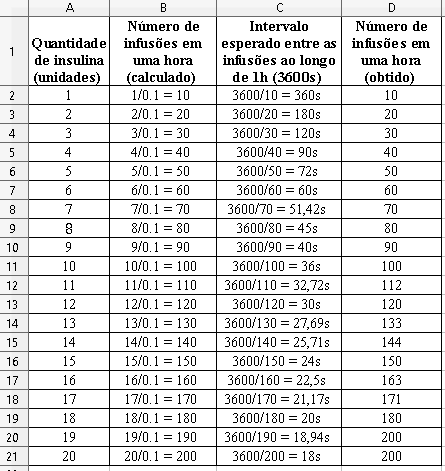
\includegraphics[scale=1]{images/tabela_injecao.png}
	\caption{Testes relizados e as relações de divisão}	
	\label{fig:testeinsulina}
\end{figure}

A partir desses testes foi possível constatar que nos casos em que o intervalo entre as infusões não é inteiro, o número de infusões realizadas eh superior ao que foi configurado pelo usuário. Isso é consequência da taxa constante que é utilizada para o cálculo da injeção, já que a parte inteira do intervalo tem maior influência sobre o resultado e não existe uma compensação para o tempo mínimo desconsiderado pela precisão limitada. Para diminuir essa diferença de injeção o sistema trata internamente todas as unidades como inteiro e utiliza-se da escala 0.1, quantidade mínima de infusão, apenas para exibir pinformações para o usuário. Isso inclusive é uma vantagem para caso seja necessário altera esse valor mínimo no futuro, pois na maioria dos módulos do sistema, se não for todos, não será necessário a alteração.

Um possível solução seria alterar a precisão do Timer do sistema e contar os décimos, centésimos ou milésimos de segundos ao invés de segundos como é feito hoje. Como consequência teria-se o aumento da precisão e a bomba poderia considerar intervalos menores para injeção.

Com isso, mostra-se que a precisão do intervalo de infusão que a bomba considera é importantíssimo, pois pode causar difereça entre a quantidade de insulina deseja e a realmente injetada, o que representa um risco ao usuário.

\section{Simulador}

O uso do simulador foi importantíssimo para o desenvolvimento desse trabalho. Ele possibilitou iniciar o desenvolvimento sem uma placa física. Utilizando-o montou-se um circuito exemplo utilizando o microcontrolador escolhido e, de forma iterativa, era possível evoluir tanto o circuito quanto o software, por exemplo: montou-se o circuito com o LCD e implementou-se o módulo de controle do mesmo, adicionou-se os componentes de menu e a análise de botões, e outros passos. Vendo esses passos é possível perceber que o desenvolvimento foi feito por funcionalidade isoladas de forma que fosse possível testar cada "parte" do software e assim minimizar os problemas do software como um todo e assim sempre ter um versão estável, mesmo que mínima.

Além de todas essas facilidades, a gama de testes e depuração é maior em um simulador do que no \emph{hardware}, como: o simulador indica más práticas existentes, permite simular o uso da bomba por dias em questão de minutos, basta configurar o tempo de execução, e outros. Graças aos exemplos citados anteriormente foi possível encontrar diversos problemas que só seriam descobertos quando estivesse testando diretamente no hardware e mesmo assim ficaria a dúvida: É o \emph{hardware} ou o \emph{software}.

Quanto ao esquema elétrico utilizado no simulador, ele foi adotado devido ao fato que os componentes utilizados serão os mesmo. Dessa forma todos os testes e validações do \emph{hardware} pelo simulador são extremamente válidas e importantes.

\section{Arquitetura modularizada}

A forma com que foi organizado o código é a grande vantagem desse trabalho. O desacoplamento foi o foco principal durante todo o desenvolvimento isso para facilitar mudanças no próprio \emph{software} ou mudança do \emph{hardware}

Utilizando OOC foi tudo pensado para que fosse possível fazer testes, mocks no sistema. Devido a forma com que foi implementado, foi possível realizar testes utilizando um PC. Foi utilizado um Ubuntu 13.10, compilador gcc, Framework C++ Qt e IDE QtCreator. Como o conceito de OOC é baseado em ponteiros de função o mock das funções foi feito apenas apontando para uma função que foi criada de acordo com a cituação de teste desejada. Quanto o acesso aos periféricos, todos os acionamentos e comunicações foram redirecionadas para um arquivo log de acompanhamento. A seguir será descrito as vantagens principais de cada módulo devido a forma de implementação.

O módulo Config é o mais simples de todos, Sua principal vantagem é o fato de centralizar todas as informações de configuração, fazendo com que o sistema fique mais claro. Além disso, criar casos de testes torna-se simples, pois mudando qualquer uma de suas informações já se reflete no sistema com um todo. É importante lembrar também que ele não carrega nenhuma dependência do compilador ou do hardware, foi implemnetado em ANSI-C, o que permite que seja utilizado por qualquer compilador e \emph{hardware}.

Os demais módulos foram criados para seguir a ideia de isolação do módulo config. Para isso o que foi feito é deixar as interfaces e funções comuns independente de \emph{hardware} e compilador utilizando apenas ANSI-C. Dessa forma, caso precise de alguma mudança mais drástica relacionada aos dois itens citados o impacto seja mínimo, precisando fazer apenas um de-para das funcionalidades específicas. 

Tendo dito as vantagens com reláção à mudanças \emph{hardware} e compilador é importante lembrar que a expansibilidade e manutenabilidade do software ficou incrivelmente simples. A ideia foi deixar o "motor" ou "coração" da bomba ter conhecimento apenas das "ïnterface" do sistemas. Dessa forma os detalhes de funcionamento, requisitos de segurança, configurações específicas de hardware para controle dos periféricos e outros, podem ser modificadas sem impactar o funcionamento básico da bomba de infusão. O mais importante é que essas alterações são parametrizável,se localizam no módulo config, e o software sabe quais objetos utilizar e de onde recuperá-los, em algum \emph{Factory} na maioria dos casos. Devido a isso tudo é possível manter mais de um produto em um único código e mudanças importantes no \emph{core} do sistema não precisa ser replicadas e correr risco de conflito entre projetos. Graças ao uso do OOC para criar algo novo basta implementar as funções da interface do módulo em questão e adicionar ao \emph{factory}, caso exista. Segue uma breve explicação do que pode ser feito em cada módulo.

O módulo InsulinPump, responsável por abstrair particularidades de funcionalidades e segurança do bomba para o resto do ambiente permite que se crie varios tipos de bomba. Essa criação leva em conta mudanças nos dois itens citados, por exemplo, bomba européia, americana, brasileira, que podem ter requisitos de segurança distintos.

O módulo LCD, responsável por abstrair a forma de uso e qual \emph{display} está sendo utilizado. Ele permite a troca do tipo de LCD utilizado seja simples, por exemplo, trocar o utiliza 2x16, por um 2x12.

O módulo Menu, lembra uma máquina de estado retorna um próximo Menu(estado) ou ele mesmo caso a mudança não ocorra. Para adiconar um novo menu é só adicionar como retorno em alguma situação dentro da função de análise de botões que todos os Menus possuem.

O módulo Motor segue a mesma linha do LCD, permite a troca do periférico por outro motor de passo ou até mesmo um outro tipo de motor.

O módulo TimerMotor foi criado para desvincular o timer que é extremamente dependente do \emph{hardware} e compilador. Foi o módulo mais complicado de se isolar e é o único que não está totalmente isolado devido a algumas limitações do execução de interrupções.